\documentclass[14pt, a4paper]{extarticle}



\usepackage{ upgreek }
\usepackage{ amssymb }

\usepackage{graphicx}
\graphicspath{{./images/}}
\DeclareGraphicsExtensions{.jpg,.png}
\usepackage{csvsimple}
 
\usepackage{amsfonts}
\usepackage{amsmath}
 
\usepackage[english,russian]{babel}
 
\usepackage{fontspec} 
\defaultfontfeatures{Ligatures={TeX},Renderer=Basic}
\setmainfont[Ligatures={TeX,Historic}]{Times New Roman}
\setmonofont{Courier New}
\newfontfamily\cyrillicfonttt[Script=Cyrillic]{Courier New}
 
\usepackage{xcolor}
 
\usepackage{array}
\newcommand\ChangeRT[1]{\noalign{\hrule height #1}}
 
\usepackage{tabularx}
\newcolumntype{s}{>{\raggedright\arraybackslash}X}
%\renewcommand{\tabularxcolumn}[1]{m{#1}} % Вертикальное нтрирование текста
 
\usepackage{indentfirst} %отступ первой строки первого абзаца
\linespread{1.25}
 
\usepackage{geometry}
\geometry{left=3cm}
\geometry{right=1cm}
\geometry{top=2cm}
\geometry{bottom=2cm}
 
\setlength{\parindent}{1.25cm}
 
\usepackage{enumitem}
\setlist{left=\parindent, labelsep=1cm, itemsep=0pt, topsep=0pt}
 
\usepackage[final]{pdfpages}
 
\usepackage{titlesec} % оформление заголовков
 
\titleformat{\section}[block]
    {\newpage\bfseries\fontsize{18pt}{21.6pt}\selectfont}
        {\thesection}
        {1em}{}
\titleformat{name=\section,numberless}[block]
    {\newpage\bfseries\fontsize{18pt}{21.6pt}\selectfont}
        {}
        {0em}{}{}
\titlespacing{\section}
 {\parindent}% space at the left
 {0em}% space before
 {10mm}% space after
\titleformat{\subsection}[block]
    {\bfseries\hspace{\parindent}\fontsize{16pt}{19.2pt}\selectfont}
        {\thesubsection}
        {1em}{}
 
\usepackage{etoolbox}
 
\usepackage{nameref}
\usepackage{hyperref}
\hypersetup{
    colorlinks,
    citecolor=black,
    filecolor=black,
    linkcolor=black,
    urlcolor=black
}
\urlstyle{same}
        
\usepackage{float}
\usepackage{caption}
 
\usepackage{newfloat}
\DeclareCaptionType[name=Листинг, placement=htbp]{listing}
 
\usepackage{fancyvrb}
 
\DeclareCaptionLabelSeparator{emdash}{\;\textemdash\;}
\captionsetup[figure]{name={Рисунок}, labelsep=emdash, justification=centering, position=above, singlelinecheck=off, font={small, bf}, labelfont=bf, skip=6pt}
\captionsetup[table]{name={Таблица}, labelsep=emdash, justification=raggedright, position=top, singlelinecheck=off, font={small, it}, labelfont=it, skip=6pt, margin=0.6cm}
\captionsetup[listing]{name={Листинг}, labelsep=emdash, justification=raggedright, position=top, singlelinecheck=off, font={small, it}, labelfont=it, skip=-16pt, margin=0.6cm}
 
\counterwithin{figure}{section}
\counterwithin{table}{section}
\counterwithin{listing}{section}
 
\usepackage{ragged2e}
\usepackage{microtype}
 
\justifying
\sloppy
\tolerance=500
\hyphenpenalty=10000 % отключение переноса
\emergencystretch=3em
 
\usepackage{setspace}
 
\usepackage{multirow}
 
\usepackage[
citestyle=gost-numeric,
style=gost-numeric, 
backend=biber
]{biblatex}
\addbibresource{kurs.bib}
%\usepackage{calc}
%\defbibenvironment{bibliography}
%  {\list{\printfield[labelnumberwidth]{labelnumber}}
%    {\setlength{\leftmargin}{\parindent}%
%     \setlength{\itemindent}{\parindent}%
%     \setlength{\labelsep}{1.5em}%
%     \addtolength{\itemindent}{\labelsep+\labelnumberwidth}%
%     \setlength{\itemsep}{\bibitemsep}%
%     \setlength{\parsep}{\bibparsep}}}
%  {\endlist}
%  {\item}
 
\usepackage{pdflscape}

\begin{document}

\makeatletter
\renewcommand{\l@section}{\@dottedtocline{1}{0em}{1.25em}}
\renewcommand{\l@subsection}{\@dottedtocline{2}{0em}{1.75em}}
\renewcommand{\l@subsubsection}{\@dottedtocline{3}{0em}{2.6em}}
\renewcommand{\@dotsep}{1.25}
\makeatother

\def\contentsname{СОДЕРЖАНИЕ}

\pagenumbering{gobble}
\begin{titlepage}
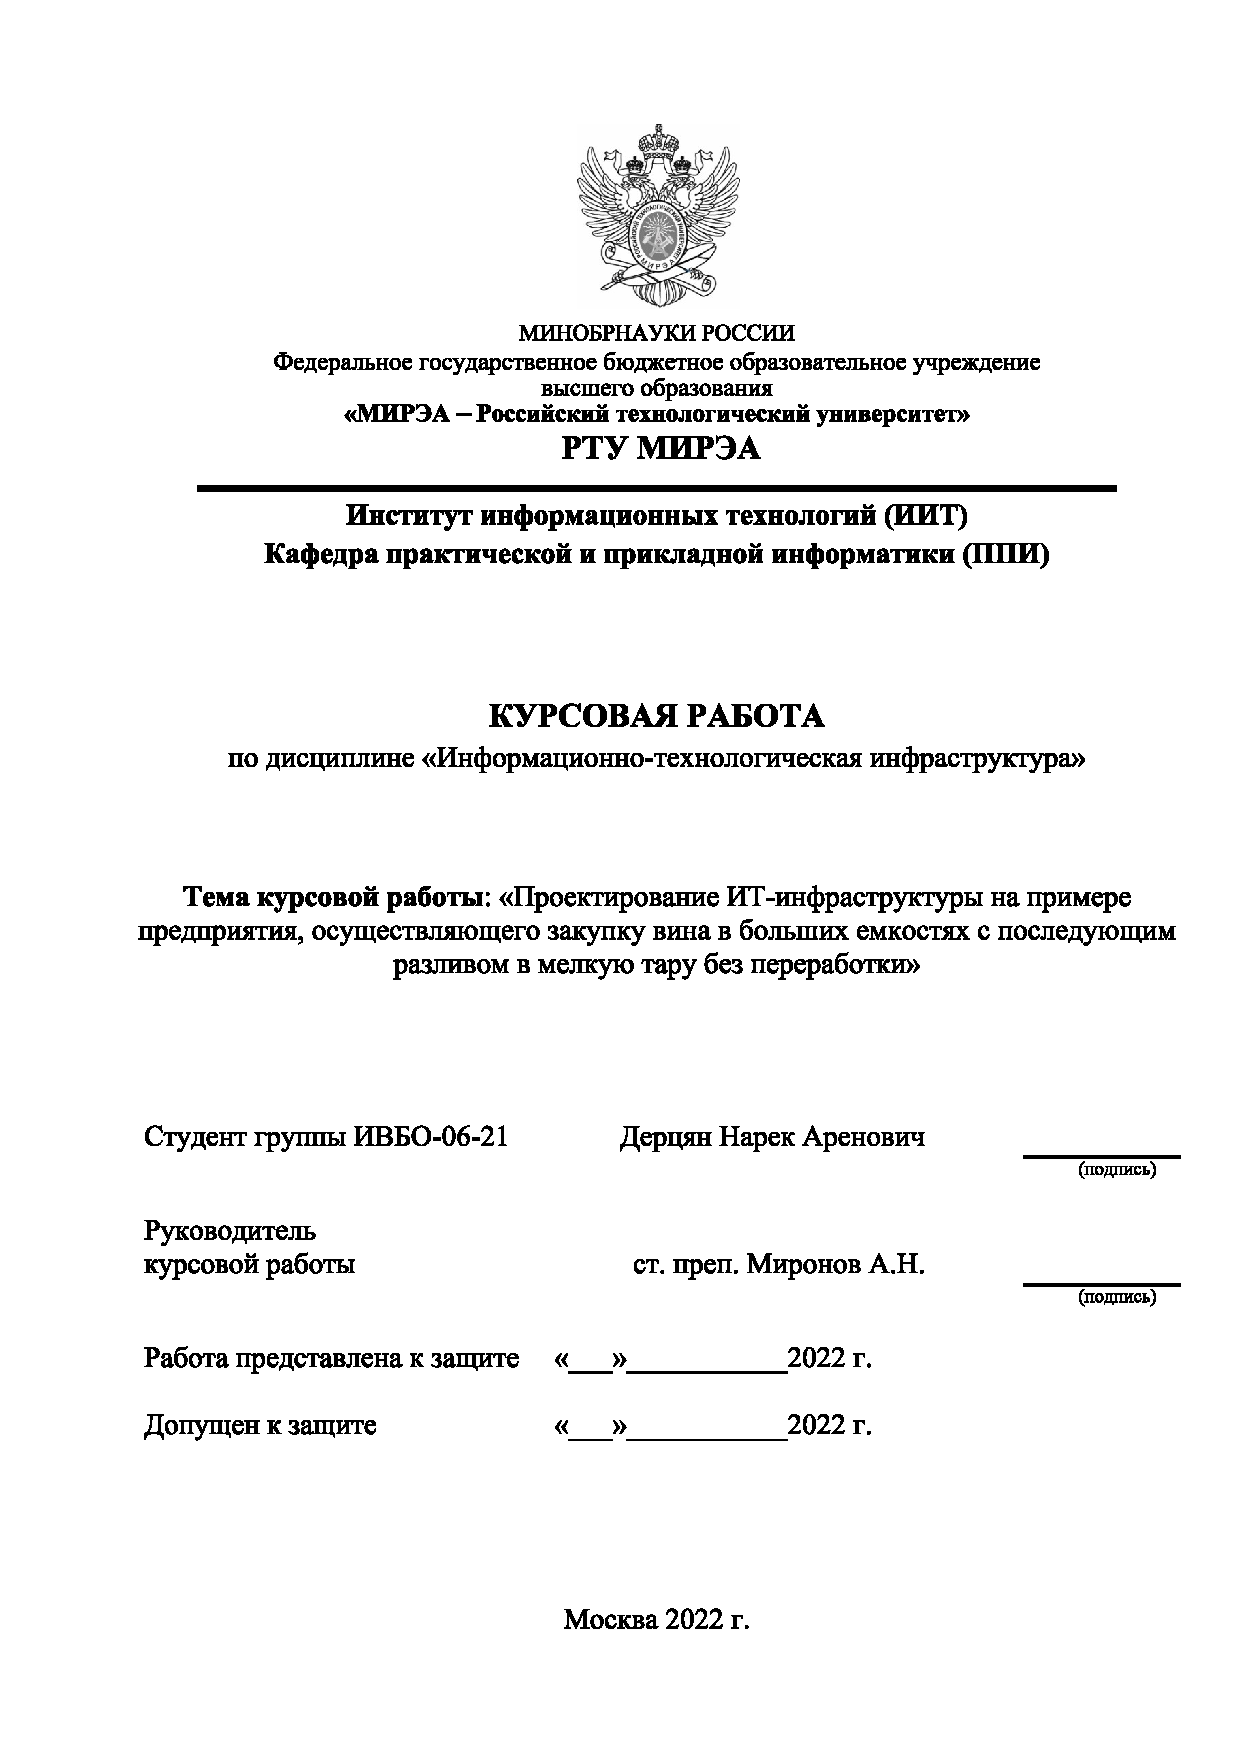
\includepdf{titleITI}
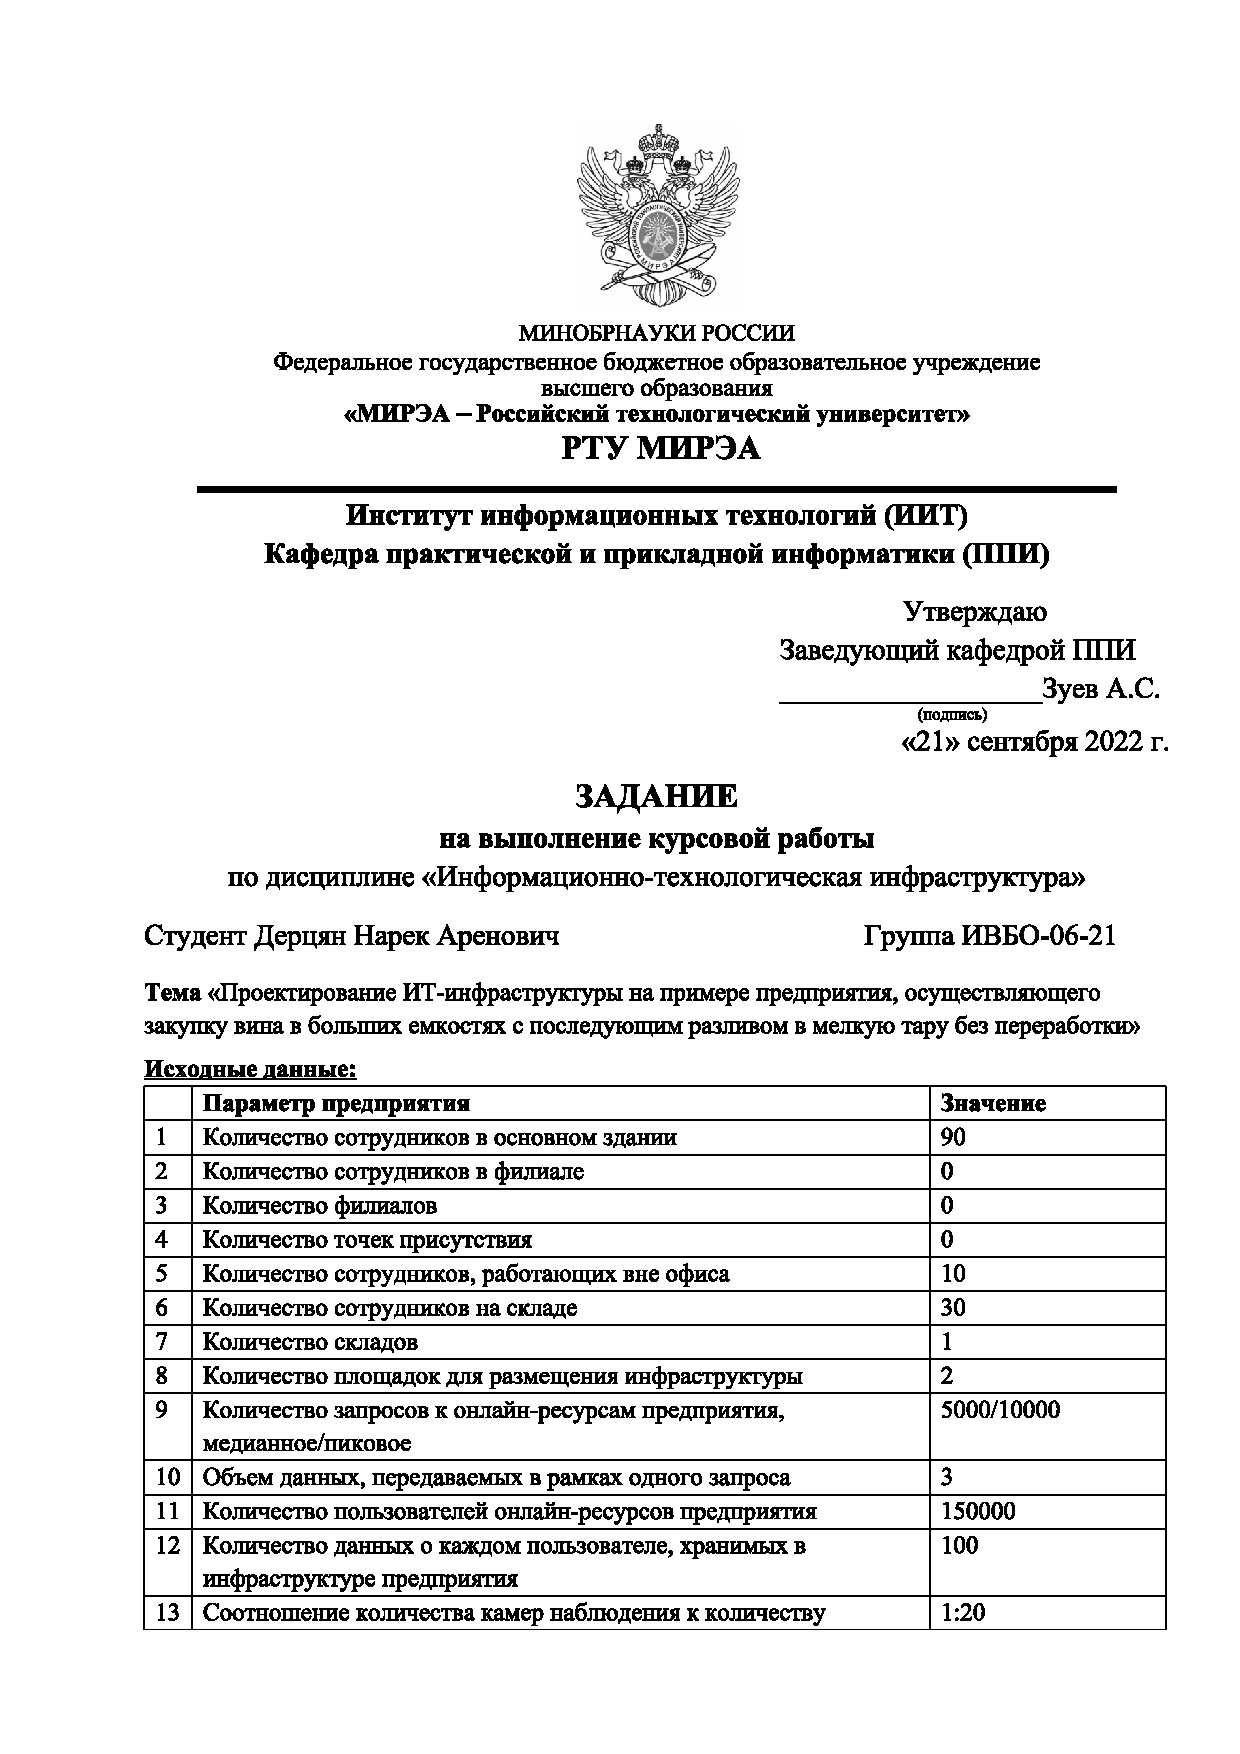
\includepdf{titletakITI}
\end{titlepage}
\tableofcontents

\section*{ВВЕДЕНИЕ}
\pagenumbering{arabic}
\setcounter{page}{3}
\addcontentsline{toc}{section}{ВВЕДЕНИЕ} % это чтобы в содержании отображалось

Данная курсовая работа посвящена проектированию информационно-технологической 
инфраструктуры на примере предприятия, осуществляющего закупку вина в больших
емкостях с последующим разливом в мелкие тары без переработки\cite{kurs-metod}.

Предприятие состоит из:
\begin{itemize}
    \item Основного здания (штаб-квартиры), в котором находятся:
        \begin{enumerate}
            \item Руководство предприятия
            \item Бухгалтерия
            \item Отдел кадров
            \item Отдел закупок
            \item Административно-хозяйственная служба
            \item ИТ-отдел
            \item Служба безопасности
        \end{enumerate}
    \item Сотрудников, работающих вне офиса
        \begin{enumerate}
            \item профильные специалисты одного из отделов штаб-квартиры или 
                  филиала. В таком случае они включаются в численность 
                  сотрудникв
                  штаб-квартиры или соответствующего филиала; 
        \end{enumerate}
    \item Сотрудников, работающих вне офиса.
        \begin{enumerate}
            \item профильные специалисты одного из отделов штаб-квартиры или 
                филиала. В таком случае они включаются в численность 
                сотрудников штаб-квартиры или соответствующего филиала
        \end{enumerate}

    \item Складов, в которых находятся
        \begin{enumerate}
            \item Руководства склада
            \item Сотрудники склада
            \item Сотрудники службы безопасности
        \end{enumerate}

\end{itemize} 

Во многом, внедрение ИТ-инфраструктуры явно способствует развитию и
росту компании. Для осуществления деятельности организациинеобходимо
внедрение ИТ-инфраструктуры для упрощения «бытовых» процессов, таких как
ведение различного учета, например, бухгалтерского, для общего документоборота и
т.п.

\section[СПЕЦИФИКАЦИЯ ОСНОВНЫХ И ВСПОМОГАТЕЛЬНЫХ БИЗНЕС-ПРОЦЕССОВ ПРЕДМЕТНОЙ ОБЛАСТИ]{СПЕЦИФИКАЦИЯ ОСНОВНЫХ И \\ВСПОМОГАТЕЛЬНЫХ БИЗНЕС-ПРОЦЕССОВ ПРЕДМЕТНОЙ ОБЛАСТИ}

Бизнес-процессы – это всё то, что происходит в компании. При этом каждый такой процесс имеет отношение в равной степени к работникам компании и её клиентам, потому что конечная цель каждой компании – создавать ценности для клиента. 

Виды бизнес процессов:
\begin{enumerate}
    \item Основным бизнес-процессом является, например, производство продукции, также в зависимости от самого бизнеса основными бизнес-процессами могут являться продажа товаров или услуг. Иными словами основной бизнес-процесс -- это процесс, который формирует цену, в том числе добавочную, какому-либо продукту за который платит клиент.  
%    \item Основным бизнес-процессом, как правило, является производство продукции/оказание услуг. Неразрывно связанным с ним и также основным бизнес-процессом является продажа товаров/услуг.
    \item Всопомогательные бизнес-процессы исходя из самого названия не нужны в бизнесе сами по себе, но без них невозможна основная и дополнительная деятельность. К таким процессам можно отнести закупку сырья, оборудования или ведение бухгалтерии.
%    \item Вспомогательные бизнес-процессы потому так и называются, что не нужны компании сами по себе, однако без них невозможна основная и дополнительная деятельность. Для подавляющего большинства компаний вспомогательные процессы – это закупка сырья и оборудования, ведение бухгалтерии, кадровая политика.
\end{enumerate}

Исходя из начальных условий, составим таблицы спецификации безнес-процессов предприятия (Таблица\;\ref{tab:buisness_spec}), спецификации пользователей (Таблица\;\ref{tab:user_spec}) и спецификации площадок размещения оборудования (Таблица\;\ref{tab:place_spec}).



\begin{landscape}
\begin{table}[H]
\caption{Спецификация бизнес-процессов предприятия\label{tab:buisness_spec}}
\centering
\small
\begin{tabularx}{700pt}{|l|>{\hsize=1\hsize}s|>{\hsize=1\hsize}s|>{\hsize=1\hsize}s|>{\hsize=1\hsize}s|>{\hsize=1\hsize}s|}
\hline
    № & Бизнес-процессы & Тип процесса & Участники (акторы) процесса & Используемое программное обеспечение & Критичность \cr \hline
    1 & Закупка товара & Основной & Специалист по закупкам & 1С:Управление торговлей, Micrasoft office, Micrasoft exchange  & Высокая \cr \hline
    2 & Администрирование системы & Вспомогательный & IT-специалист & 1C:EDT, Ansible, Zabbix, Acronis, PostgreSQL & Средняя \cr \hline
    3 & Управление компанией & Вспомогательный & Генеральный директор, Заместитель директора & 1С:Управление нашей компнией, Micrasoft 365 office, Ivideon, МойСклад, Micrasoft exchange & Очень высокая \cr \hline
    4 & Административно-хозяйственная служба & Вспомогательный & Уборщики, электрик, сантехник & Micrasoft exchange, Micrasoft 365 office & Средняя \cr \hline
    5 & Охрана помещений & Вспомогательный & Охранник & Ivideon, МойСклад, Micrasoft exchange, Micrasoft 365 office & Средняя \cr \hline
    6 & Бухгалтерское обеспечение & Вспомогательный & Бухгалтер & 1С:Бухгалтерия,  Micrasot exchange, Micrasoft 365 office & Средняя \cr \hline
    7 & Кадровое обеспечение & Вспомогательный & Сотрудник отдела кадров & 1С:Зарплата и управление персоналом, Micrasot exchange, Micrasoft office 365 & Низкая \cr \hline
    8 & Управление складом & Вспомогательный & Заведующий складом & МойСклад, Micrasoft 365 office, Micrasoft exchange & Средняя \cr \hline
\end{tabularx}
\end{table}
\end{landscape}



\begin{landscape}
\begin{table}[H]
\caption{Спецификация пользователей\label{tab:user_spec}}
\centering
\small
\begin{tabularx}{700pt}{|c|s|s|s|s|s|s|}
\hline
    № & Тип пользователя & Количество пользователей & Участие в бизнес-процессах & Используемый интерфейс & Требования к программному обеспечению на рабочем месте & Рабочее место расположено: \cr \hline
    1 & Генеральный директор & 1 & Управление компанией & Персональный компьютер, мобильное приложение & Micrasoft 365 office, Micrasoft exchange, 1С:Управление нашей фирмой & Основное здание \cr \hline
    2 & Заместители директоров & 6 & Управление компанией & Персональный компьютер,  мобильное приложение & Браузер, Micrasoft 365 office, Micrasoft exchange, 1С:Управление нашей фирмой & Основное здание и филиалы \cr \hline
    3 & Бухгалтер & 18 & Бухгалтерское обеспечение & Персональный компьютер & Micrasoft 365 office, 1С:Бухгалтерия, Браузер & Основное здание \cr \hline
    4 & Сотрудник склада & 20 & Прием и приходование товара & Терминал сбора данных, мобильное приложение & МойСклад, Micrasoft exchange, Micrasoft 365 office & Склад \cr \hline
    5 & Сотрудник cлужбы безопасности & 25 & Обеспечение безопасности & Персональный компьютер, мобильное приложение & Micrasoft exchange, Браузер, Система видеонаблюдения, система связи & Основное здание, склад \cr \hline
    6 & Сотрудник отдела закупок & 25 & Заключение договоров о поставках & Персональный компьютер, мобильное приложение & 1С:Управление торговлей, Браузер, Micrasoft 365 office, Micrasoft exchange & Основное здание \cr \hline
\end{tabularx}
\end{table}


\begin{table}[H]
\caption*{Продолжение таблицы\;\ref{tab:user_spec}}
\centering
\small
\begin{tabularx}{700pt}{|c|s|s|s|s|s|s|}
\hline
    7 & Сотрудник отдела кадров & 18 & Кадровое обеспечение & Персональный компьютер, мобильное приложение & Браузер, Micrasoft 365 office, Micrasoft exchange, мессенджеры, 1С:Зарплата и управление персоналом & Основное здание \cr \hline
    8 & Сотрудник административно-хозяйственной службы & 8 & Обслуживание помещений & Мобильное приложение & Axmor & Основное здание, склад \cr \hline
    9 & Сотрудник IT-службы & 10 & Техническое обслуживание, разработка & Персональный компьютер, мобильное приложение & 1C:EDT, Ansible, Браузер, Zabbix, Acronis, PostgreSQL & Основное здание, вне офиса \cr \hline
    10 & Пользователь онлайн-ресурса предприятия & 15000 & Продажа пива & Персональный компьютер, мобильное приложение & Веб-сайт & Вне офиса \cr \hline
\end{tabularx}
\end{table}
\end{landscape}






\begin{landscape}
\begin{table}[H]
\caption{Спецификация площадок размещения оборудования\label{tab:place_spec}}
\centering
\small
\begin{tabularx}{600pt}{|c|s|s|s|s|s|}
\hline
        № & Площадка & Количество площадок & Энергоснабжение & Перечень провайдеров и скорость каналов связи & Количество АРМ сотрудников \cr \hline
        1 & Штаб квартира (Ул. лобачевского 88) & 1 & 2 ввода 35Квт & Ростелеком (500 Мбит/с), МТС (300 Мбит/с) & 75 \cr \hline
        2 & Склад (Ул. Лермонтова 3) & 1 & 3 ввода по 25Квт & Ростелеком (500 Мбит/с), МТС (300 Мбит/с) & 16 \cr \hline
        3 & Площадки для размещения инфраструктуры & 2 & 3 входа по 60Квт &  Ростелеком (20 Гбит/с), МТС (10 Гбит/с) & 0 \cr \hline
\end{tabularx}
\end{table}
\end{landscape}

\section[СПЕЦИФИКАЦИЯ СЕРВИСОВ, РАЗЕРТЫВАЕМЫХ В ИНФРАСТРУКТУРЕ, С УКАЗАНИЕМ ВЕРСИЙ ПРИКЛАДНОГО ПРОГРАММНОГО ОБЕСПЕЧЕНИЯ]{СПЕЦИФИКАЦИЯ СЕРВИСОВ, \\РАЗЕРТЫВАЕМЫХ В ИНФРАСТРУКТУРЕ, С УКАЗАНИЕМ ВЕРСИЙ ПРИКЛАДНОГО \\ПРОГРАММНОГО ОБЕСПЕЧЕНИЯ}


Прикладное программное обеспечение делится на три основных класса:
\begin{itemize}
    \item Устанавливаемое на АРМ пользователя;
    \item Устанавливаемое на серверах предприятия;
    \item Получаемое в качестве облачной подписки на какой-либо сервис. 
\end{itemize}

Исходя из полученных данных, а также сведений, содержащихся в спецификации на выбранное программное обеспечение заполним таблицы со спецификацией\cite{system-requirments} прикладного ПО\cite{sites} на АРМ пользователей (Таблица\;\ref{tab:prog_spec}), спецификацией прикладного ПО на серверах (Таблица\;\ref{tab:servProg_spec}) и спецификацией подписок на облачные сервисы (Таблица\;\ref{tab:clouds}). Для видеонаблюдения будем пользоваться сервисом облачного видеонаблюдения VSAASI\cite{vsaas}, так-как такм сопобом можно сократить количество систем хранения данных.


\begin{landscape}
\begin{table}[H]
\caption{Спецификация прикладного ПО на АРМ пользователей\label{tab:prog_spec}}
\centering
\small
\begin{tabularx}{700pt}{|l|>{\hsize=1\hsize}s|>{\hsize=1.15\hsize}s|>{\hsize=1.15\hsize}s|>{\hsize=0.7\hsize}s|>{\hsize=1\hsize}s|>{\hsize=1\hsize}s|>{\hsize=1\hsize}s|}
\hline
    № & Название ПО, версия & Функционал & Тип пользователя & Количество установок & Тип лицензии и цена одной единицы & Потребление ресурсов (Процессор/ ОЗУ/ Диск) & Тип ОС \cr \hline

        1 & Micrasoft office 365, 2021 & Офисное приложение & Все сотрудники, использующее АРМ & 70 & Платная, 10000 рублей 6 установок & Версия Windows 7 и новее, процессор х32/х64 с тактовой частотой 1Ггц, 2Гб ОЗУ, 3Гб жесткий диск & Windows \cr \hline

        2 & 1C:EDT, 2022.1 & Прикладные решения & IT- специалист & 10 & Бесплатно & Процессор intel 2Ггц и выше, 2Гб ОЗУ для 32-х битной ОС или 4Гб ОЗУ для 64-х битной ОС, жесткий диск 500Мб или выше & Windows/Linux \cr \hline

        3 & МойCклад, 2022 & Складской учет & Сотрудник склада & 18 & Платная, 32215 рублей в месяц одна установка & Windows 7 и выше, процессор от 2Ггц, ОЗУ от 4Гб, жесткий диск 2Гб & Windows/ Linux/ ios /Android \cr \hline
        4 & 1C:Управление нашей фирмой, 8.3 & Управление предприятием & Генеральный директор, заместитель директора & 7 & Платная, 5400 рублей & intel 2Ггц х64, ОЗУ 4Гб, жеcткий диск 500Мб & Windows \cr \hline
\end{tabularx}
\end{table}

\begin{table}[H]
\caption*{Продолжение таблицы\;\ref{tab:prog_spec}}
\centering
\small
\begin{tabularx}{700pt}{|l|>{\hsize=1\hsize}s|>{\hsize=1.15\hsize}s|>{\hsize=1.15\hsize}s|>{\hsize=0.7\hsize}s|>{\hsize=1\hsize}s|>{\hsize=1\hsize}s|>{\hsize=1\hsize}s|}
%\begin{tabularx}{700pt}{|c|s|s|s|s|s|s|s|}
\hline

        5 & 1C:Бухгалтерия, 8.6 & Управление бухгалтерией & Бухгалтер & 18 & Платная, 14400 руб & x32 или x64 совместимый процессов c тактовой частотой более 2 ГГц, от 4 Гб ОЗУ, от 40 Гб дискового пространства  & Windows  /  Linux \cr \hline
        6 & 1С:Управление торговлей, 11.3 & Управление закупками и торговлей & Сотрудник отдела закупок & 25 & Платная, 22600 рублей & Процессор с поддержкой intel 64, х64 или х86, ОЗУ 4 Гб и больше, жесткий диск 40Гб & Windows \cr \hline
        %6 & Ivideon, 3.12.0 & Система видеонаблюдения и связи & Охранная служба, IT- специалист & 35 & Платная, 2990 за одну камеру & Архитектура с разрядностью 32 или 64 бит, Процесcор 1,5 Ггц и выше, ОЗУ 0,5Гб и больше, жесткий диск 1Гб и больше & Windows/ Linux/ macOS \cr \hline
        7 & 1C:Зарплата и управление персоналом, 8.3 & Кадровое упраление & Сотрудник отдела кадров & 18 & Платная, 8100 рублей &  x32 или x64 совместимый процессор c тактовой частотой более 2 ГГц, от 4 Гб ОЗУ, от 40 Гб дискового пространства & Windows  \cr \hline
        8 & Яндекс браузер, 22.1.0.2510 & Браузер & Все сотрудники & 120 & Бесплатная & Windows 7 или новее, Intel pentium 4 или выше, жесткий диск 400 Мб и больше, 512 Мб ОЗУ & Windows / macOS \cr \hline
\end{tabularx}
\end{table}

\begin{table}[H]
\caption{Спецификация прикладного ПО на серверах\label{tab:servProg_spec}}
\centering
\small
\begin{tabularx}{700pt}{|l|>{\hsize=1\hsize}s|>{\hsize=1.2\hsize}s|>{\hsize=1.4\hsize}s|>{\hsize=0.95\hsize}s|>{\hsize=0.85\hsize}s|>{\hsize=0.9\hsize}s|>{\hsize=1\hsize}s|>{\hsize=0.7\hsize}s|}
\hline
    № & Название ПО, версия & Функционал & Тип пользователя & Количество пользователей & Количество установок & Тип лицензии и цена одной единицы & Потребление ресурсов Процессор/ ОЗУ/ Диск & Тип ОС \cr \hline
    
        1 & Acronis, 5.6.0 & Система управления резервными копиями & IT-спецталист & 10 & 4 & Платная, 3000 рублей в месяц & Для Windows 2Гб ОЗУ и более, процессор с частотой 2Ггц и более, жесткий диск 3Гб и более & Windows / Linux \cr \hline % Везде дописать тип лицензии и доделать пару ласт пунктов

        2 & Zabbix, 6.2 & Система мониторинга & IT- специалист & 10 & 4 & Бесплатная & 16-ти и больше ядерный процессор, 64Гб жесткий диск & Linux \cr \hline

        %3 & MySQL Server, 8.0 & База данных & IT- Специалист & 10 & 4 & Платная, 455820 рублей5+ сокетов & 4-х ядерный процессор, 8Гб ОЗУ или больше, 1.5Гб жесткий диск, RAID10 или RAID 0+1 & Windows / Linux \cr \hline
        %3 & Percona Server, 8.0 & Набор инструментов для администрирования БД & IT- Специалист & 10 & 4 & Бесплатно & 2 или больше потоков процессора на узел, 2Гб ОЗУ или, 60Гб жесткий диск или больше & Linux \cr \hline 
        3 & 1С: Предприятие, 8.6 & Управление предприятием & Генеральный директор, директор филиала, заместитель директора,  сотрудники отделов закупок и кадров  & 59 & 4 & Платная, 6300 рублей & x32 или x64 совместимый процессов c тактовой частотой более 2 ГГц, от 4 Гб ОЗУ, от 40 Гб дискового пространства  & Windows  /  Linux \cr \hline
\end{tabularx}
\end{table}

\begin{table}[H]
\caption*{Продолжение таблицы\;\ref{tab:servProg_spec}}
\centering
\small
%\begin{tabularx}{700pt}{|c|s|s|s|s|s|s|s|}
\begin{tabularx}{700pt}{|l|>{\hsize=1\hsize}s|>{\hsize=1.2\hsize}s|>{\hsize=1.4\hsize}s|>{\hsize=0.95\hsize}s|>{\hsize=0.85\hsize}s|>{\hsize=0.9\hsize}s|>{\hsize=1\hsize}s|>{\hsize=0.7\hsize}s|}
\hline


        4 & PostgreSQL, 15 & Свободная Объектно-Реляционная Система Управления Базами Данных &   IT- Специалист & 10 & 4 & Бесплатно & Двухъядерный процессор 1Ггц или больше, 2Гб ОЗУ, 2Гб жесткий диск, RAID1 & Linux \cr \hline
\end{tabularx}
\end{table}


\begin{table}[H]
\caption{Спецификация подписок на облачные сервисы\label{tab:clouds}}
\centering
\small
%\begin{tabularx}{700pt}{|c|s|s|s|s|s|s|s|}
\begin{tabularx}{700pt}{|l|>{\hsize=1\hsize}s|>{\hsize=1\hsize}s|>{\hsize=1\hsize}s|>{\hsize=1\hsize}s|>{\hsize=1\hsize}s|}
\hline
    № & Название ПО & Функционал & Тип пользователя & Количество пользователей & Способ тарификации и тариф \cr \hline
    1 & Ansible & Система управления конфигурациями & IT-Специалист управляющий серверами & 1 & Бесплатно \cr \hline

    2 & micrasoft 365 office & Офисное приложение & Все сотрудники работающие на АРМ & 120 & Платная, 3000 в месяц за каждого пользователя \cr \hline

    3 & TorGuard & VPN сервис & IT-Специалист & 10 & Платная, 5480 в год \cr \hline
    4 &  VSAASI    & Сервис облачного видеонаблюдения        &  Сотрудник службы охраны, сотрудник склада   &  55  & Платная, 1400 рублей в месяц \cr \hline
\end{tabularx}
\end{table} 
\end{landscape}


\section[СПЕЦИФИКАЦИЯ СИСТЕМНОГО ПРОГРАММНОГО \\ОБЕСПЕЧЕНИЯ, С УКАЗАНИЕМ ВЕРСИЙ ПРОГРАММНОГО ОБЕСПЕЧЕНИЯ]{СПЕЦИФИКАЦИЯ СИСТЕМНОГО \\ПРОГРАММНОГО ОБЕСПЕЧЕНИЯ, С УКАЗАНИЕМ ВЕРСИЙ ПРОГРАММНОГО ОБЕСПЕЧЕНИЯ}


Системное программное обеспечение — программы, решающие задачи общевычислительного характера — вы­де­ле­ния и разделения ресурсов, доступа к устройствам, обеспечивающие среды для разработки, запуска и выполнения других про­грамм.

Системное программное обеспечение определяется исходя из потребностей
пользователей в прикладном программном обеспечении, для обеспечения его запуска.


Системное программное обеспечение делится на три основных класса:
\begin{enumerate}
    \item Устанавливаемое на АРМ пользователя;
    \item Устанавливаемое на серверах предприятия;
    \item Получаемое по модели IAAS или PAAS в облаке. 
\end{enumerate}

    Исходя из полученных данных, а также сведений, содержащихся в спецификации на выбранное программное обеспечение заполним таблицы со спецификацией системного ПО на АРМ пользователей (Таблица\;\ref{tab:sys_prog_spec}), спецификацией системного ПО на серверах (Таблица\;\ref{tab:sys_servProg_spec}) и перечнем подписок на облачные сервисы (Рисунок\;\ref{tab:clouds-2}). Сайт предприятия будет поддерживаться на сервисe для работы с веб приложениями Selectel\cite{selectel} в целеях сокращения количества оборудования.


\begin{landscape}
\begin{table}[H]
\caption{Спецификация системного ПО на АРМ пользователей\label{tab:sys_prog_spec}}
\centering
\small
\begin{tabularx}{700pt}{|l|>{\hsize=1\hsize}s|>{\hsize=1\hsize}s|>{\hsize=1\hsize}s|>{\hsize=0.6\hsize}s|>{\hsize=1\hsize}s|>{\hsize=1.4\hsize}s|}
\hline
    № & Название ПО, версия & Функционал & Тип пользователя & Количество установок & Тип лицензии и цена одной единицы & Потребление ресурсов (Процессор/ ОЗУ/ Диск) \cr \hline

        1 & Windows 11 & Операционная система & Все АРМ & 130 & Платная, 5000 рублей за одну установку & Двухъядерный процессор с тактовой частотой 1ГГци выше, 4 Гб ОЗУ, 64 Гб жесткий диск, видеокарта с поддержкой DirectX 12 \cr \hline

        2 & Ubuntu, 22.04.1 LTS & Операционная система & IT- специалист & 10 & Бесплатно & Двухъядерный процессор с тактовой частотой 2 ГГц или выше, 4 Гб ОЗУ, 25 Гб свободного пространства на жестком диске \cr \hline

        3 & Android 13 & Операционная система для мобильных девайсов & Сотрудник склада, сотрудник административно-хозяйственного отдела & 35 & Бесплатно & x86 или х64 процессор / не менее 2 ГБ оперативной / не менее 16 ГБ встроенной памяти \cr \hline
\end{tabularx}
\end{table}



\begin{table}[H]
\caption{Спецификация системного ПО на серверах предприятия\label{tab:sys_servProg_spec}}
\centering
\small
\begin{tabularx}{700pt}{|l|>{\hsize=1\hsize}s|>{\hsize=1\hsize}s|>{\hsize=0.6\hsize}s|>{\hsize=1\hsize}s|>{\hsize=1.4\hsize}s|}
\hline
    № & Название ПО, версия & Функционал & Количество установок & Тип лицензии и цена одной единицы & Потребление ресурсов (Процессор/ ОЗУ/ Диск) \cr \hline

%        1 & Windows Server 2019 & Операционная система & 1 & Платная, 5000 рублей за одну установку & Процессор64-разрядный процессор с частотой 1,4 ГГц. Совместимость с набором инструкций x64 Поддержка NX и DEP. Поддержка CMPXCHG16b, LAHF/SAHF и PrefetchW \cr \hline

        1 & Ubuntu Server, 22.04.1 LTS & Операционная система & 2 & Бесплатно & Двухъядерный процессор с тактовой частотой 2 ГГц или выше, 4 Гб ОЗУ, 25 Гб свободного пространства на жестком диске \cr \hline

        2 & Ansible & Система управления конфигурациями & 2 & Бесплатно & 32- или 64-разрядный X86-процессор с тактовой частотой не менее 1,0 ГГц / От 2 ГБ оперативной памяти /3 ГБ свободного пространства на жестком диске \cr \hline
\end{tabularx}
\end{table}






\begin{table}[H]
\caption{Спецификация подписок на облачные сервисы\label{tab:clouds-2}}
\centering
\small
%\begin{tabularx}{700pt}{|c|s|s|s|s|s|s|s|}
\begin{tabularx}{700pt}{|l|>{\hsize=1\hsize}s|>{\hsize=1\hsize}s|>{\hsize=1\hsize}s|>{\hsize=1\hsize}s|}
\hline
    № & Название ПО & Функционал & Количество пользователей & Способ тарификации и тариф \cr \hline

    1 & Selectale  & Инфраструктура для работы веб-приложений & 16 core/32 ОЗУ/ 390 локальный диск  & Платно, 18000 рублей в месяц\cr \hline
\end{tabularx}
\end{table} 
\end{landscape}



\section[РАСЧЕТ ПРОИЗВОДСТВЕННОГО АППАРАТНОГО ОБЕСПЕЧЕНИЯ, НЕОБХАДИМОГО ДЛЯ ФУНКЦИОНИРОВАНИЯ ОПИСАННЫХ СЕРВИСОВ, И ВЫБОР СРЕДСТВ И ПОДХОДОВ К ВИРТУАЛИЗАЦИИ И ПОСТРОЕНИЮ ВЫЧИСЛИТЕЛЬНОГО КЛАСТЕРА, \\ОБЛАДАЮЩЕГО НЕОБХАДИМОЙ ПРОИЗВОДИТЕЛЬНОСТЬЮ]{РАСЧЕТ ПРОИЗВОДСТВЕННОГО \\АППАРАТНОГО ОБЕСПЕЧЕНИЯ, НЕОБХАДИМОГО ДЛЯ ФУНКЦИОНИРОВАНИЯ ОПИСАННЫХ СЕРВИСОВ, И ВЫБОР СРЕДСТВ И ПОДХОДОВ К ВИРТУАЛИЗАЦИИ И ПОСТРОЕНИЮ \\ВЫЧИСЛИТЕЛЬНОГО КЛАСТЕРА, \\ОБЛАДАЮЩЕГО НЕОБХАДИМОЙ \\ПРОИЗВОДИТЕЛЬНОСТЬЮ}

В этом разделе представлены карточки требований к АРМ пользователей
(таблицы\;\ref{tab:card_dir}-\ref{tab:card_IT}) и вычислительному кластеру на базе ОС Ubuntu Server (таблица\;\ref{tab:card_server}).



\begin{table}[H]
\caption{Карточка требований к АРМ пользователя <<Генеральный директор>>\label{tab:card_dir}}
\centering
\small
\begin{tabularx}{450pt}{|l|s|s|}
\hline
    № & Тип пользователя & Генеральный директор \cr \hline
    1 & Используемая ОС & Windows 11 для ПК и Android 13 для смартфона \cr \hline
    2 & Прикладное ПО & Micrasoft 365 office, Micrasoft exchange, 1С:Управление нашей фирмой, Яндекс браузер \cr \hline
    3 & Суммарный минимальный требуемый объем хранилища, ГБ & 90 Гб для ПК и 32 для смартфона \cr \hline
    4 & Суммарный минимальный объем ОЗУ для запуска самого производительного приложения и самой ОС, ГБ & 8 для ПК и 4 для смартфона \cr \hline
    5 & Требования к CPU и GPU  & На менее 2-х ядер, х64 для ПК и MediaTek Helio G35 на смартфон \cr \hline
    6 & Форм-фактор & ПК, смартфон \cr \hline
    7 & Подключение к сети  & 500 Мб/с \cr \hline
\end{tabularx}
\end{table}


\begin{table}[H]
\caption{Карточка требований к АРМ пользователя <<Заместитель директора>>\label{tab:card_zam_dir}}
\centering
\small
\begin{tabularx}{450pt}{|l|s|s|}
\hline
    № & Тип пользователя & Заместитель директора \cr \hline
    1 & Используемая ОС & Windows 11 для ПК и Android 13 для смартфона \cr \hline
    2 & Прикладное ПО &  Micrasoft 365 office, Micrasoft exchange, 1С:Управление нашей фирмой, Яндекс браузер \cr \hline
    3 & Суммарный минимальный требуемый объем хранилища, ГБ & 90 Гб для ПК и 32 для смартфона \cr \hline
    4 & Суммарный минимальный объем ОЗУ для запуска самого производительного приложения и самой ОС, ГБ & 8 для ПК и 4 для смартфона \cr \hline
    5 & Требования к CPU и GPU  & На менее 2-х ядер, х64 для ПК и MediaTek Helio G35 на смартфон \cr \hline
    6 & Форм-фактор & ПК, смартфон \cr \hline
    7 & Подключение к сети  & 500 Мб/с \cr \hline
\end{tabularx}
\end{table}


\begin{table}[H]
\caption{Карточка требований к АРМ пользователя <<Сотрудник отдела закупок>>\label{tab:card_otdel_zakupk}}
\centering
\small
\begin{tabularx}{450pt}{|l|s|s|}
\hline
    № & Тип пользователя & Сотрудник отдела закупок \cr \hline
    1 & Используемая ОС & Windows 11 \cr \hline
    2 & Прикладное ПО & 1С:Управление торговлей, Micrasoft 365 office, Micrasoft exchange, Яндекс браузер \cr \hline
    3 & Суммарный минимальный требуемый объем хранилища, ГБ & 80 Гб для \cr \hline
    4 & Суммарный минимальный объем ОЗУ для запуска самого производительного приложения и самой ОС, ГБ & 8 Гб \cr \hline
    5 & Требования к CPU и GPU  & На менее 2-х ядер, х64 \cr \hline
    6 & Форм-фактор & ПК \cr \hline
    7 & Подключение к сети  & 500 Мб/с \cr \hline
\end{tabularx}
\end{table}

\begin{table}[H]
\caption{Карточка требований к АРМ пользователя <<Сотрудник отдела кадров>>\label{tab:card_kadr}}
\centering
\small
\begin{tabularx}{450pt}{|l|s|s|}
\hline
    № & Тип пользователя & Сотрудник отдела кадров\cr \hline
    1 & Используемая ОС & Windows 11 \cr \hline
    2 & Прикладное ПО & 1С: Зарплата и управление персоналом, Micrasoft 365 office, Micrasoft exchange, Яндекс браузер \cr \hline
    3 & Суммарный минимальный требуемый объем хранилища, ГБ & 32 Гб\cr \hline
    4 & Суммарный минимальный объем ОЗУ для запуска самого производительного приложения и самой ОС, ГБ & 8 Гб \cr \hline
    5 & Требования к CPU и GPU  & На менее 2-х ядер, х64 \cr \hline
    6 & Форм-фактор & ПК \cr \hline
    7 & Подключение к сети  & 500 Мб/с \cr \hline
\end{tabularx}
\end{table}

\begin{table}[H]
\caption{Карточка требований к АРМ пользователя <<Сотрудник склада>>\label{tab:card_sklad}}
\centering
\small
\begin{tabularx}{450pt}{|l|s|s|}
\hline
    № & Тип пользователя & Сотрудник склада\cr \hline
    1 & Используемая ОС & Android 13 \cr \hline
    2 & Прикладное ПО & Micrasoft 365 office, Micrasoft exchange, МойСклад, браузер \cr \hline
    3 & Суммарный минимальный требуемый объем хранилища, ГБ & 32 Гб\cr \hline
    4 & Суммарный минимальный объем ОЗУ для запуска самого производительного приложения и самой ОС, ГБ & 8 Гб \cr \hline
    5 & Требования к CPU и GPU  & MediaTek Helio G35 \cr \hline
    6 & Форм-фактор & Смартфон/ терминал сбора данных \cr \hline
    7 & Подключение к сети  & 300 Мб/с \cr \hline
\end{tabularx}
\end{table}


\begin{table}[H]
\caption{Карточка требований к АРМ пользователя <<Сотрудник службы безопасности>>\label{tab:card_oxrana}}
\centering
\small
\begin{tabularx}{450pt}{|l|s|s|}
\hline
    № & Тип пользователя & Сотрудник службы безопасности \cr \hline
    1 & Используемая ОС & Windows 11 \cr \hline
    2 & Прикладное ПО & Micrasoft 365 office, Micrasoft exchange, браузер \cr \hline
    3 & Суммарный минимальный требуемый объем хранилища, ГБ & 70 Гб\cr \hline
    4 & Суммарный минимальный объем ОЗУ для запуска самого производительного приложения и самой ОС, ГБ & 8 Гб \cr \hline
    5 & Требования к CPU и GPU  & На менее 2-х ядер, х64 \cr \hline
    6 & Форм-фактор & ПК \cr \hline
    7 & Подключение к сети  & 300 Мб/с \cr \hline
\end{tabularx}
\end{table}

\begin{table}[H]
\caption{Карточка требований к АРМ пользователя <<Бухгалтер>>\label{tab:card_buxgalter}}
\centering
\small
\begin{tabularx}{450pt}{|l|s|s|}
\hline
    № & Тип пользователя & Бухгалтер \cr \hline
    1 & Используемая ОС & Windows 11 \cr \hline
    2 & Прикладное ПО & Micrasoft 365 office, Micrasoft exchange, браузер, 1С:Бухгалтерия \cr \hline
    3 & Суммарный минимальный требуемый объем хранилища, ГБ & 70 Гб\cr \hline
    4 & Суммарный минимальный объем ОЗУ для запуска самого производительного приложения и самой ОС, ГБ & 8 Гб \cr \hline
    5 & Требования к CPU и GPU  & На менее 2-х ядер, х64 \cr \hline
    6 & Форм-фактор & ПК \cr \hline
    7 & Подключение к сети  & 500 Мб/с \cr \hline
\end{tabularx}
\end{table}



\begin{table}[H]
\caption{Карточка требований к АРМ пользователя <<IT-Специалист>>\label{tab:card_IT}}
\centering
\small
\begin{tabularx}{450pt}{|l|s|s|}
\hline
    № & Тип пользователя & IT-Специалист \cr \hline
    1 & Используемая ОС & Windows 11, Ubuntu 22.04.1 LTS \cr \hline
    2 & Прикладное ПО & Micrasoft 365 office, Micrasoft exchange, браузер, 1C:EDT, Ansible, Браузер, Zabbix, Acronis, PostgreSQL \cr \hline
    3 & Суммарный минимальный требуемый объем хранилища, ГБ & 200 Гб\cr \hline
    4 & Суммарный минимальный объем ОЗУ для запуска самого производительного приложения и самой ОС, ГБ & 16 Гб \cr \hline
    5 & Требования к CPU и GPU  & На менее 4-х ядер, х64 \cr \hline
    6 & Форм-фактор & ПК \cr \hline
    7 & Подключение к сети  & 500 Мб/с \cr \hline
\end{tabularx}
\end{table}


\begin{table}[H]
\caption{Карточка требований к вычислительным кластерам на базе на базе ОС Ubuntu Server 22.04.1 LTS\label{tab:card_server}}
\centering
\small
\begin{tabularx}{450pt}{|l|s|s|}
\hline
    № & Тип ОС & ОС Ubuntu Server 22.04.1 LTS \cr \hline
    1 & Системное ПО & Ansible \cr \hline
    2 & Прикладное ПО & 1С:Предприятие, Acronis, Zabbix, PostgreSQL \cr \hline
    3 & Количество экземпляров ОС & 2 \cr \hline
    4 & Суммарный минимальный требуемый объем хранилища, ГБ & 1000 Гб\cr \hline
    5 & Суммарный минимальный объем ОЗУ для запуска самого производительного приложения и самой ОС, ГБ & 80 Гб \cr \hline
    6 & Требования к CPU и GPU  & На менее 20-х ядер, х64 \cr \hline
    7 & Подключение к сети  & 20 Гб/с \cr \hline
\end{tabularx}
\end{table}


Исходя из общих требований по количеству запущенных экземпляров ОС, а
также надежности и отказоустойчивости, можем построить топологию
развертывания (Рисунок\;\ref{fig:topology}), а также составить карточки кластеров\cite{trinity} (таблицы\;\ref{tab:kl-1}, \;\ref{tab:res-1}).


\begin{figure}[H]
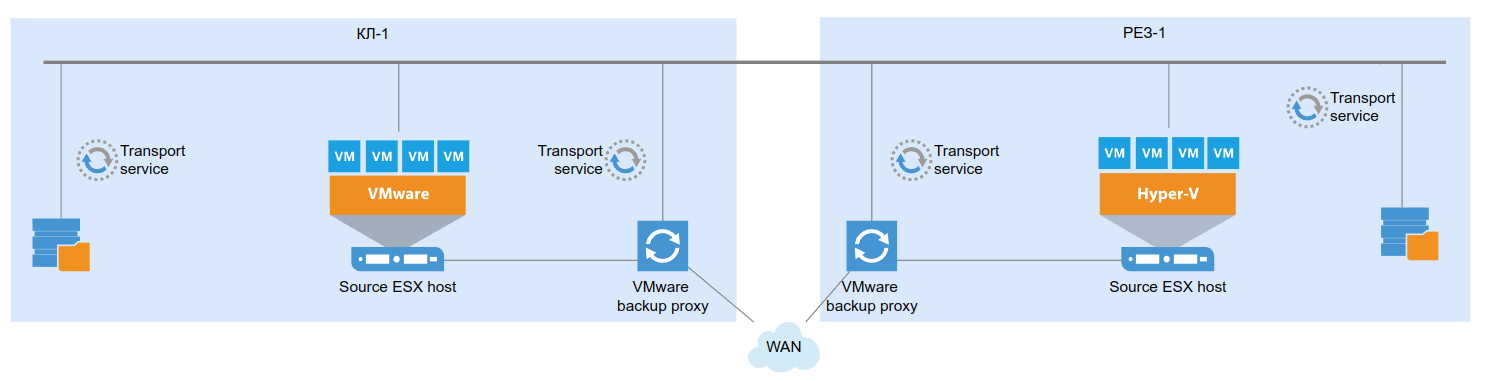
\includegraphics[scale=0.33]{topology.png}
\caption{Топология развертывания инфраструктуры\label{fig:topology}}
\end{figure}


\begin{table}[H]
\centering
\small
\caption{Карточка кластероа (узла) КЛ-1\label{tab:kl-1}}
\begin{tabular}{|l|lll|}
\hline
\multicolumn{1}{|c|}{№} & \multicolumn{1}{l|}{Тип гипервизора}                                                      & ProMox                  &        \\ \hline
1                       & \multicolumn{1}{l|}{Количество VM}                                                        & 4                       &        \\ \hline
%2                       & \multicolumn{1}{l|}{Количество контейнеров, тип}                                          & \multicolumn{1}{l|}{45} & Docker \\ \hline
3                       & \multicolumn{1}{l|}{\begin{tabular}[c]{@{}l@{}}Суммарный минимальный требуемый\\ объем хранилища, ГБ\end{tabular}}                                                                                                                                                & 600                     &        \\ \hline
4                       & \multicolumn{1}{l|}{\begin{tabular}[c]{@{}l@{}}Суммарный минимальный объем ОЗУ\\ для запуска всех приложений, ГБ\end{tabular}}                                                                                                                                    & 64                      &        \\ \hline
5                       & \multicolumn{1}{l|}{Требования к CPU и GPU}                                               & Не менее 11 ядер, x64   &        \\ \hline
6                       & \multicolumn{1}{l|}{Подключение к сети}                                                   & 20 Гбит/с               &        \\ \hline
7                       & \multicolumn{1}{l|}{Количество аппаратных узлов}                                          & 2                       &        \\ \hline
8                       & \multicolumn{3}{l|}{конфигурация аппаратного узла  <<1U/8 Cores/96 GB RAM DDR3, 650 Вт>>}                                    \\ \hline
8.1                     & \multicolumn{1}{l|}{Корпус}                                                               & \multicolumn{1}{l|}{Quanta 1U, 4HS, 650Вт}                                                                                                                                                      & 1      \\ \hline
    8.2                     & \multicolumn{1}{l|}{Материнская плата}                                                & \multicolumn{1}{l|}{\begin{tabular}[c]{@{}l@{}}Quanta, 2xLGA 2011, \\16xDDR3 Reg, PCI-e, 2xGbit, IP-KVM\end{tabular}}                                                                           & 1      \\ \hline
        8.3                     & \multicolumn{1}{l|}{Процессор}                                                    & \multicolumn{1}{l|}{\begin{tabular}[c]{@{}l@{}}Intel Xeon E5-2650v2 (2.6GHz - \\3.4GHz, 20Mb, 8 cores)\end{tabular}}                                                                            & 2      \\ \hline
8.4                     & \multicolumn{1}{l|}{Оперативная память}                                                   & \multicolumn{1}{l|}{16 GB DDR3 ECC REG}                                                                                                                                                         & 4      \\ \hline
8.5                     & \multicolumn{1}{l|}{Raid контролер}                                                       & \multicolumn{1}{l|}{\begin{tabular}[c]{@{}l@{}}LSI MegaRAID SAS 9361-4i,\\ 12Gb/s, 1GB, 4-port\end{tabular}}                                                                                    & 1      \\ \hline
8.6                     & \multicolumn{1}{l|}{Жесткие диски}                                                        & \multicolumn{1}{l|}{1 TB SATA Enterprise HDD}                                                                                                                                                   & 7      \\ \hline
9                       & \multicolumn{1}{l|}{Цена одного узла, руб}                                                        & 196000          &        \\ \hline
\end{tabular}
\end{table}


\begin{table}[H]
\centering
\small
\caption{Карточка кластера (узла) РЕЗ-1\label{tab:res-1}}
\begin{tabular}{|l|lll|}
\hline
\multicolumn{1}{|c|}{№} & \multicolumn{1}{l|}{Тип гипервизора}                                                      & ProMox                  &        \\ \hline
1                       & \multicolumn{1}{l|}{Количество VM}                                                        & 4                       &        \\ \hline
%2                       & \multicolumn{1}{l|}{Количество контейнеров, тип}                                          & \multicolumn{1}{l|}{45} & Docker \\ \hline
3                       & \multicolumn{1}{l|}{\begin{tabular}[c]{@{}l@{}}Суммарный минимальный требуемый\\ объем хранилища, ГБ\end{tabular}}                                                                                                                                                & 600                     &        \\ \hline
4                       & \multicolumn{1}{l|}{\begin{tabular}[c]{@{}l@{}}Суммарный минимальный объем ОЗУ\\ для запуска всех приложений, ГБ\end{tabular}}                                                                                                                                    & 64                      &        \\ \hline
5                       & \multicolumn{1}{l|}{Требования к CPU и GPU}                                               & Не менее 11 ядер, x64   &        \\ \hline
6                       & \multicolumn{1}{l|}{Подключение к сети}                                                   & 20 Гбит/с               &        \\ \hline
7                       & \multicolumn{1}{l|}{Количество аппаратных узлов}                                          & 2                       &        \\ \hline
8                       & \multicolumn{3}{l|}{конфигурация аппаратного узла  <<1U/8 Cores/96 GB RAM DDR3, 650 Вт>>}                                    \\ \hline
8.1                     & \multicolumn{1}{l|}{Корпус}                                                               & \multicolumn{1}{l|}{Quanta 1U, 4HS, 650Вт}                                                                                                                                                      & 1      \\ \hline
    8.2                     & \multicolumn{1}{l|}{Материнских плата}                                                & \multicolumn{1}{l|}{\begin{tabular}[c]{@{}l@{}}Quanta, 2xLGA 2011, \\16xDDR3 Reg, PCI-e, 2xGbit, IP-KVM\end{tabular}}                                                                           & 1      \\ \hline
        8.3                     & \multicolumn{1}{l|}{Процессор}                                                    & \multicolumn{1}{l|}{\begin{tabular}[c]{@{}l@{}}Intel Xeon E5-2650v2 (2.6GHz - \\3.4GHz, 20Mb, 8 cores)\end{tabular}}                                                                            & 2      \\ \hline
8.4                     & \multicolumn{1}{l|}{Оперативная память}                                                   & \multicolumn{1}{l|}{16 GB DDR3 ECC REG}                                                                                                                                                         & 4      \\ \hline
8.5                     & \multicolumn{1}{l|}{Raid контролер}                                                       & \multicolumn{1}{l|}{\begin{tabular}[c]{@{}l@{}}LSI MegaRAID SAS 9361-4i,\\ 12Gb/s, 1GB, 4-port\end{tabular}}                                                                                    & 1      \\ \hline
8.6                     & \multicolumn{1}{l|}{Жесткие диски}                                                        & \multicolumn{1}{l|}{1 TB SATA Enterprise HDD}                                                                                                                                                   & 7      \\ \hline
9                       & \multicolumn{1}{l|}{Цена одного узла, руб}                                                        & 196000          &        \\ \hline
\end{tabular}
\end{table}


\section{СПЕЦИФИКАЦИЯ ХРАНИЛИЩА ДАННЫХ И УРОВЕНЬ RAID, РЕКОМЕНДУЕМЫХ К ИСПОЛЬЗОВАНИЮ}



Каждому вычислительному кластеру предоставляется требуемый объем
полезной памяти, предоставляемый системой хранения данных. Ниже представлен расчет емкости СХД (таблица\;\ref{tab:SXD_size}). Для повышения отказоустойчивости будем использовать RAID5, работающий с одним диском четности на четырех дисках с данными и с коэффициентом избыточных дисков 0,8 для дисков типа SAS. Типы дисков SATA будут работать с RAID6, у которого коэффициент избыточных дисков 0,66. RAID6 использует на четыре диска с данными два диска четности.



\begin{table}[H]
\caption{Расчет емкости СХД\label{tab:SXD_size}}
\centering
\small
\begin{tabularx}{450pt}{|l|l|s|s|s|s|}
\hline
    № & Тип данных             & Объем, Гб & Емкость и тип диска                                & Уровень RAID & Количество дисков \cr \hline
    1 & Данные пользователей   & 15012     & 2400 GB 10,000 rpm SAS12G 2.5                      & RAID5        & 7                 \cr \hline
%    2 & Данные видеонаблюдения & 2400      & 3.5 10TB Seagate Exos 7E10 / SATA 6Gb/s, 7200rpm   & RAID5        & 1                 \cr \hline
    2 & Резервные копии        & 22600     & 3.5 10TB Seagate Exos 7E10 / SATA 6Gb/s, 7200rpm   & RAID6        & 3                 \cr \hline
    & Всего данных             & 40012     &                                                    &              &                   \cr \hline
\end{tabularx}
\end{table}


\section{СПЕЦИФИКАЦИЯ ПЛАНА РАЗМЕЩЕНИЯ ОБОРУДОВНАНИЯ НА ПЛОЩАДКАХ И В СТОЙКАХ}



На основе данных, полученных из предыдущих вычислений нужно вычислить размеры\cite{trinity-storage} и количество узлов, требуемых для серверных шасси, СХД, телекоммуникационного оборудования и ИПБ (Рисунок\;\ref{rab:kol_oborudovania}). Данная таблица для <<ВМ-1>> и <<РЕP-1>> будут совпадать, так как площадки размещения инфраструктуры типовые.

\begin{table}[H]
\caption{Расчет количества оборудования\label{tab:kol_oborudovania}}
\centering
\small
\begin{tabularx}{450pt}{|l|s|s|s|}
\hline
    № & Тип оборудования                    & Высота, U & Количество узлов \cr \hline
    1 & Серверные шасси                     &    2      &       2          \cr \hline
    2 & Системы хранения данных             &    2      &       2       \cr \hline
    3 & Телекоммуникационное оборудование   &    1      &       54      \cr \hline
    4 & Источники бесперебойного питания    &    2      &       4      \cr \hline
    \multicolumn{2}{|l|}{Всего:}            &    6      &       62         \cr \hline
\end{tabularx}
\end{table}

Ниже представлен типовой план размещения оборудования в площадке
размещения инфраструктуры. Он будет общим для центров обработки данных КЛ-1
и РЕЗ-1 (Рисунки\;\ref{fig:server_plan}, \ref{fig:server_plan2}):



\begin{figure}[H]
\centering
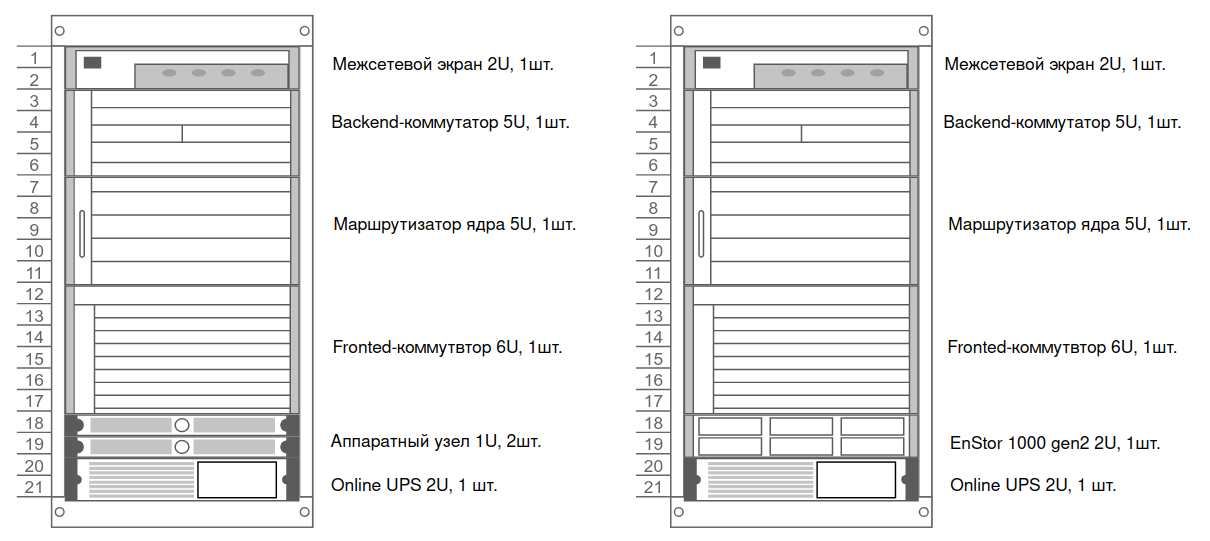
\includegraphics[scale=0.38]{server_plan1}
\caption{Плана размещения оборудования-1\label{fig:server_plan}}
\end{figure}

\begin{figure}[H]
\centering
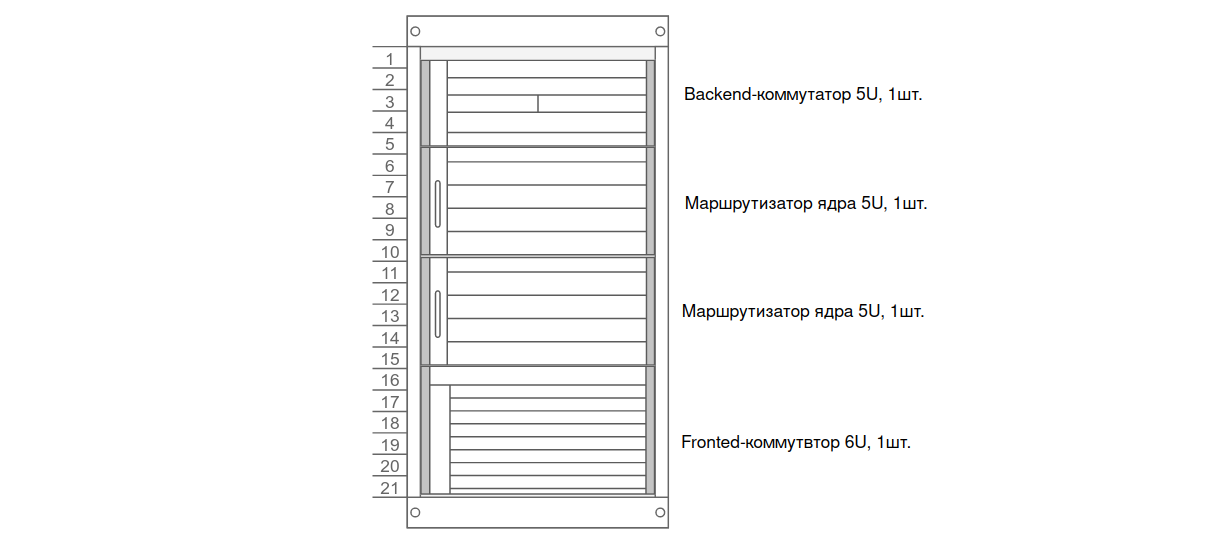
\includegraphics[scale=0.38]{server_plan2}
\caption{Плана размещения оборудования-2\label{fig:server_plan2}}
\end{figure}




Далее представлен расчет количество оборудования, присутствующего в штаб-квартире и на складе (Таблица\;\ref{tab:sostav_arm})


\begin{table}[H]
\caption{Расчет состава АРМ\label{tab:sostav_arm}}
\centering
\small
\begin{tabularx}{450pt}{|l|>{\hsize=1.1\hsize}s|>{\hsize=1\hsize}s|>{\hsize=1.4\hsize}s|s|>{\hsize=0.8\hsize}s|>{\hsize=0.7\hsize}s|}
\hline
    № & Тип пользователя & Количество АРМ & Характеристики монитора, количество & IP-телефон & Сканер & Принтер  \cr \hline
    \multicolumn{7}{|c|}{Штаб-квартира}                \cr \hline
    1 & Генеральный директор          & 1  & 1920х1080, 1 & 1  & 1 & 1 \cr \hline
    2 & Заместитель директора         & 6  & 1920х1080, 6 & 3  & 3 & 2 \cr \hline
    3 & Бухгалтер                     & 18 & 1920х1080, 18& 10 & 10& 3 \cr \hline
    4 & Сотрудник службы безопасности & 7  & 1920х1080, 2 &нет &нет&нет\cr \hline
    5 & Сотрудник отдела закупок      & 15 & 1920х1080, 15& 6  & 6 & 3 \cr \hline
    6 & Сотрудник отдела кадров       & 18 & 1920х1080, 18& 4  & 4 & 2 \cr \hline
    \multicolumn{7}{|c|}{Склад}                                        \cr \hline
    1 & Сотрудник склада              & 5  & 1920х1080, 5 & 2  & 5 & 1 \cr \hline
    2 & Сотрудник службы безопасности & 7  & 1920х1080, 2 &нет &нет&нет\cr \hline
    \multicolumn{2}{|c|}{Всего:}      & 75 &      67      & 26 &29 & 12\cr \hline
\end{tabularx}
\end{table}


Далее проведем расчет общих средств оргтехники — сетевых МФУ, проекторов, ИБП, контрольно-кассовых узлов и комплектов видеоконференцсвязи, используемых в разных частях предприятия (Таблица\;\ref{tab:sostav_arm}).



\begin{table}[H]
\caption{Расчет состава АРМ\label{tab:sostav_arm}}
\centering
\small
\begin{tabularx}{450pt}{|l|>{\hsize=1\hsize}s|>{\hsize=1\hsize}s|>{\hsize=1\hsize}s|}
\hline
    № & Тип оргтехники & Количество & Характеристики                 \cr \hline
    \multicolumn{4}{|c|}{Штаб-квартира}                \cr \hline
    1 & Сетевое МФУ                   & 3  & Мощность 56 КВт/70 КВА \cr \hline
    2 & Резервный ИБП                 & 12 & Мощность 28 Квт/35 КВА \cr \hline
    \multicolumn{4}{|c|}{Склад}                                        \cr \hline
    1 & Терминал сбора данных         & 5  & Мощность 0,04Вт/0,05 КВА  \cr \hline
    \multicolumn{2}{|c|}{Всего:}      & 20 &                         \cr \hline
\end{tabularx}
\end{table}




\section[СПЕЦИФИКАЦИЯ СЕТЕВОЙ ИНФРАСТРУКТУРЫ РЕШЕНИЯ С ОПИСАНИЕМ ПРОПУСКНОЙ СПОСОБНОСТИ ВАНАЛОВ СВЯЗИ И УЧЕТОМ ТРЕБОВАНИЙ ПО РЕЗЕРВИРОВАНИЮ И ОТКАЗАУСТИ]{СПЕЦИФИКАЦИЯ СЕТЕВОЙ \\ИНФРАСТРУКТУРЫ РЕШЕНИЯ С ОПИСАНИЕМ ПРОПУСКНОЙ СПОСОБНОСТИ ВАНАЛОВ СВЯЗИ И УЧЕТОМ ТРЕБОВАНИЙ ПО РЕЗЕРВИРОВАНИЮ И ОТКАЗАУСТИ}


На основе данных рассчитанных в предыдущих пунктах составим общую схему отображающую связь всех компонентов ИТ-инфраструктуры между собой (Рисунок\;\ref{fig:network})



\begin{figure}[H]
\centering
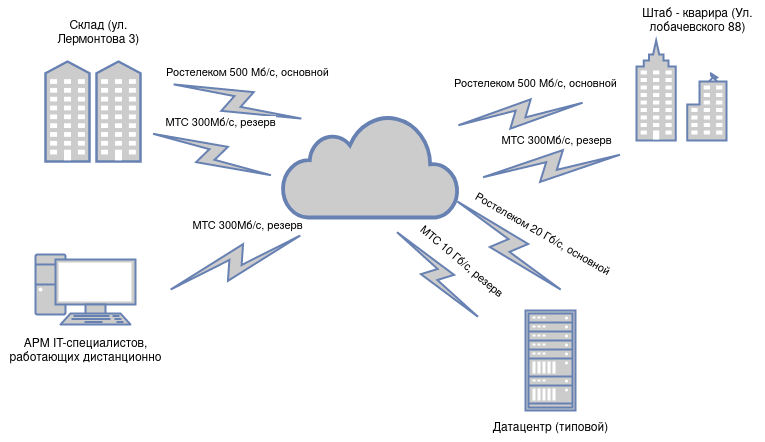
\includegraphics[scale=0.6]{network.png}
\caption{Общая топология сети предприятия\label{fig:network}}
\end{figure}


Исходя из количества рабочих мест, приведем расчет емкости портов коммуникаторов и их количества (Рисунок\;\ref{tab:coumunication})

\begin{table}[H]
\caption{Спецификация телекоммуникационного оборудования\label{tab:coumunication}}
\centering
\small
\begin{tabularx}{450pt}{|l|>{\hsize=1.2\hsize}s|>{\hsize=0.8\hsize}s|s|s|s|s|}
\hline
    № & Тип оборудования & Высота, u & Количество портов & Количество & Мощность, КВТ  \cr \hline
    1 & Межсетевой экран           & 2 & 24 & 2  & 0,15 \cr \hline
    2 & Маршрутизатор              & 1 & 4  & 2  & 0,8  \cr \hline
    3 & Коммутатор ядра            & 1 & 2  & 2  & 0,5  \cr \hline
    4 & Коммутатор распределения   & 1 & 28 & 4  & 0,26 \cr \hline
    \multicolumn{4}{|c|}{Всего:}            & 10 & 1,71 \cr \hline
    \multicolumn{6}{|c|}{Склад}                         \cr \hline
    1 & Маршрутизатор              & 1 & 4  & 2  & 0,8  \cr \hline
    2 & Роутер                     & 1 & 6  & 5  & 0,4  \cr \hline
    \multicolumn{4}{|c|}{Всего:}            & 7  & 1,2  \cr \hline
\end{tabularx}
\end{table}



Ниже показаны схемы сети для таких компонентов предприятия, как штаб-квартира (Рисунок\;\ref{fig:comp_net}) и склад (Рисунок\;\ref{fig:sklad_net}). На складе будем использовать WIFI-роутер так-как большинство сотрудников склада используют терминалы для сбора данных, для которых обязательно наличие WIFI.  

\begin{figure}[H]
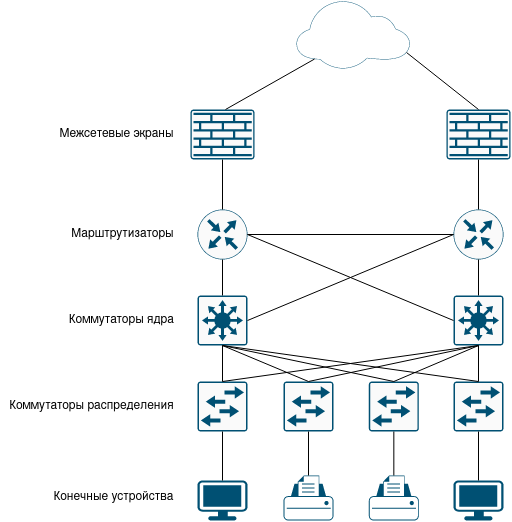
\includegraphics[scale=0.65]{comp_network.png}
\caption{Cхема сети штаб-квартиры\label{fig:comp_net}}
\end{figure}


\begin{figure}[H]
\centering
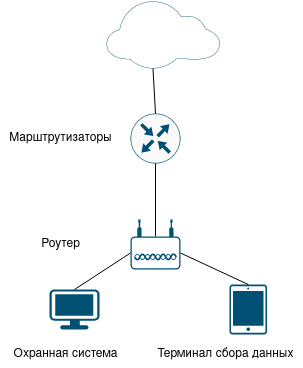
\includegraphics[scale=0.75]{sklad_net.png}
\caption{Cхема сети склада\label{fig:sklad_net}}
\end{figure}

Далее представлена схема сети центра обработки данных (Рисунок\;\ref{fig:server_network}) и таблица со спецификацией телекоммуникационного оборудования (Таблица\;\ref{tab:serv_comunication}) Для обеспечения надежности и отказоустойчивости применим дублирование ключевых узлов и каналов связи данной сети. Схемы сетей для ЦОД КЛ-1 и РЕЗ-1 одинаковы и считаются типовыми.




\begin{table}[H]
\caption{Спецификация телекоммуникационного оборудования центра обработки данных\label{tab:serv_comunication}}
\centering
\small
\begin{tabularx}{450pt}{|l|>{\hsize=1.2\hsize}s|>{\hsize=0.8\hsize}s|s|s|s|s|}
\hline
    № & Тип оборудования & Высота, u & Количество портов & Количество & Мощность, КВТ  \cr \hline
    \multicolumn{6}{|c|}{Штаб-квартира}                     \cr \hline
    1 & Межсетевой экран           & 2  & 4     & 2  & 0,8  \cr \hline
    2 & Маршрутизатор ядра         & 5  & 5     & 4  & 0,15 \cr \hline
    3 & Frontend коммутатор        & 6  & 30    & 3  & 1,6  \cr \hline
    4 & Beckend коммутатор         & 4  & 28    & 3  & 1,3  \cr \hline
    \multicolumn{2}{|c|}{Всего:}   & 54 &  202  & 12 & 46,2 \cr \hline
\end{tabularx}
\end{table}


\begin{figure}[H]
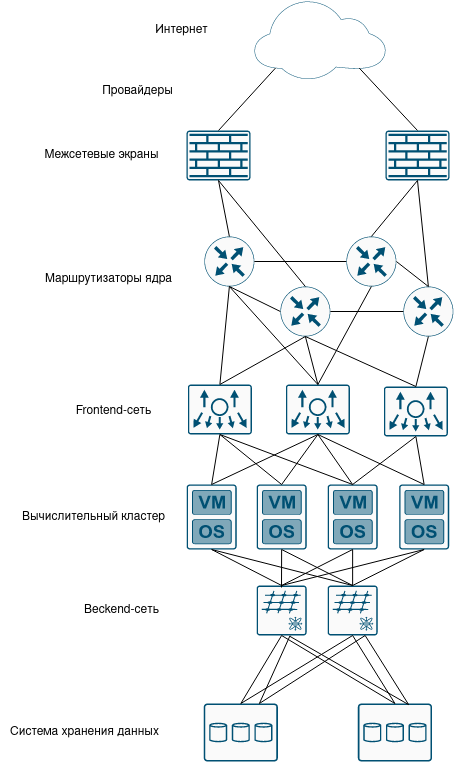
\includegraphics[scale=0.75]{server_network.png}
\caption{Схема сети центра обработки данных (типовая)\label{fig:server_network}}
\end{figure}


\section[СПЕЦИФИКАЦИЯ ТЕХНИЧЕСКОГО ОБЕСПЕЧЕНИЯ, \\НЕОБХАДИМОГО ДЛЯ РАЗЕРТЫВАНИЯ ДАННОЙ \\ИНФРАСТРУКТУРЕ: СИСТЕМ ЭЛЕКТРОСНАБЖЕНИЯ, ВЕНТИЛЯЦИИ И КОНДИЦИРОВАНИЯ, ПОЖАРОТУШЕНИЯ]{СПЕЦИФИКАЦИЯ ТЕХНИЧЕСКОГО \\ОБЕСПЕЧЕНИЯ, НЕОБХАДИМОГО \\ДЛЯ РАЗЕРТЫВАНИЯ ДАННОЙ \\ИНФРАСТРУКТУРЕ: СИСТЕМ \\ЭЛЕКТРОСНАБЖЕНИЯ, ВЕНТИЛЯЦИИ И КОНДИЦИРОВАНИЯ, ПОЖАРОТУШЕНИЯ}


Проведем расчет потребляемой оборудованием мощности по площадке. При этом учтем АРМ, их компоненты, устройства оргтехники и прочее телекоммуникационное оборудование (Таблица\;\ref{tab:potreblya}).

\begin{table}[H]
\caption{Расчет потребляемой оборудованием мощности на площадке\label{tab:potreblya}}
\centering
\small
\begin{tabularx}{450pt}{|l|>{\hsize=1.5\hsize}s|>{\hsize=0.8\hsize}s|s|s|>{\hsize=0.7\hsize}s|}
\hline
    № & Тип оргтехники & Количество & Мощность, КВт & Мощность, КВА & cos $u$ \cr \hline
    \multicolumn{6}{|c|}{Штаб-квартира}                                \cr \hline
    1 & Сетевое МФУ                       & 2  & 0,55  & 0,825   & 0,8 \cr \hline
    2 & АРМ                               & 90 & 0,35  & 0,4375  & 0,8 \cr \hline
    3 & Комплект видеоконференцсвязи      & 20 & 0,046 & 0,0575  & 0,8 \cr \hline
    4 & Камеры видеонаблюдения            & 5  & 0,03  & 0,0375  & 0,8 \cr \hline
    \multicolumn{2}{|c|}{Всего:}          & 117& 33,67 & 42,0875 &     \cr \hline
    \multicolumn{6}{|c|}{Склад}                                        \cr \hline
    1 & Терминал сбора данных             & 10 &  0,04 &  0,05   & 0,8 \cr \hline
    2 & Камеры видеонаблюдения            & 3  &  0,03 &  0,04   & 0,8 \cr \hline
    3 & АРМ                               & 10 &  0,35 &  0,4375 & 0,8 \cr \hline
    \multicolumn{2}{|c|}{Всего:}          & 13 &  0,79 &  1      &     \cr \hline
\end{tabularx}
\end{table}


На основе данных расчётов посчитаем количество ИБП, необходимое для данной площадки (Таблица\;\ref{tab:ibp}).

\begin{table}[H]
\caption{Расчет ИБП по площадкам \label{tab:ibp}}
\centering
\small
\begin{tabularx}{450pt}{|l|>{\hsize=1.2\hsize}s|>{\hsize=0.8\hsize}s|s|s|}
\hline
    № & Тип ИБП & Тип АРМ пользователя & Количество & Мощность, КВА    \cr \hline
    \multicolumn{5}{|c|}{Штаб-квартира}                                \cr \hline
    1 & ИБП резервного типа           & ПК & 12 & 3,5         \cr \hline
    2 & ИБП с двойным преобразованием & ПК & 4  & 10          \cr \hline
    \multicolumn{3}{|c|}{Всего:}           & 3  & 82          \cr \hline
\end{tabularx}
\end{table}

\begin{table}[H]
\caption*{Продолжение таблицы \;\ref{tab:ibp}}
\centering
\small
\begin{tabularx}{450pt}{|l|>{\hsize=1.2\hsize}s|>{\hsize=0.8\hsize}s|s|s|}
\hline
    \multicolumn{5}{|c|}{Склад}                               \cr \hline
    1 & ИБП резервного типа           & Терминал сбора данных/ПК & 3  & 0,6         \cr \hline
    2 & ИБП с двойным преобразованием & Терминал сбора данных/ПК & 2  & 0,9        \cr \hline
    \multicolumn{3}{|c|}{Всего:}           &  3,6 &  4,5        \cr \hline
\end{tabularx}
\end{table}




Далее представлены расчеты потребляемой мощности, количества ИБП, системы охлаждения\cite{temp-metod} и системы пожаротушения\cite{fire-metod} ЦОД КЛ-1 (Таблицы\;\ref{tab:power} -\;\ref{tab:cooler2}). Эти же значения применяются и к ЦОД РЕЗ-1:



\begin{table}[H]
\caption{Расчет потребляемой оборудованием мощности в ЦОД КЛ-1 (типовой)\label{tab:power}}
\centering
\small
\begin{tabularx}{450pt}{|l|>{\hsize=1.7\hsize}s|>{\hsize=0.9\hsize}s|s|s|>{\hsize=0.4\hsize}s|}
\hline
    № & Тип техники & Количество & Мощность, кВт/ч & Мощность, КВА & cos $u$         \cr \hline
    1 & Телекоммуникационное оборудование      & 1 & 46,2 &57,75 & 0,8\cr \hline  
    2 & Узел 1U/8 Cores/96 GB RAM DDR3, 650 Вт & 2 & 0,65 & 0,75 & 0,8\cr \hline
\end{tabularx}
\end{table}


\begin{table}[H]
\caption{Расчет ИРП для ЦОД КЛ-1 (типовой)\label{tab:irp}}
\centering
\small
\begin{tabularx}{450pt}{|l|>{\hsize=1\hsize}s|>{\hsize=1\hsize}s|s|s|>{\hsize=1\hsize}s|}
\hline
    № & Тип ИП & Класс ИП & Тип установки & Количество & Мощность, КВА \cr \hline
    1 & ИРП & Online UPS & В стойку          &  2   & 0,8 \cr \hline  
    2 & ИБП & ДГУ        & Уличный контейнер & 1    & 50  \cr \hline
\end{tabularx}
\end{table}



К вентиляции серверной комнаты предъявляют следующие требования:

\begin{itemize}
    \item температурный режим: от +17 °C до +25 °C
    \item влажность: 40—55\%
    \item уровень запылённости помещения: в рамках 0,001 г/м$^3$
    \item уровень атмосферного давления: 85–105 кПа
    \item кратность воздухообмена в серверной: 1,5–2 крата/час
\end{itemize}



Пусть серверная комната имеет размеры 3х3х2,7 метра. Тогда воздухообменом и теплопоступлением через наружную стену можно пренебречь ввиду малых габаритов.


\begin{table}[H]
\caption{Расчет системы охлаждения для ЦОД КЛ-1 (типовой)\label{tab:cooler}}
\centering
\small
\begin{tabularx}{450pt}{|l|>{\hsize=1\hsize}s|>{\hsize=1\hsize}s|s|s|>{\hsize=1\hsize}s|}
\hline
    № & Тип источника тепла & Мощность электрическая, кВт/ч & Мощность, тепловая кВт/ч & Мощность, BTU  \cr \hline
    1 & Вычислительная техника        & 47,5 & 47,5 & 158,175 \cr \hline  
    2 & Тепловые характеристики здания & 1,3 & 1,3 & 4,329 \cr \hline
\end{tabularx}
\end{table}

\begin{table}[H]
\caption{Расчет системы пожаротушения для ЦОД КЛ-1 (типовой)\label{tab:cooler2}}
\centering
\small
\begin{tabularx}{450pt}{|l|>{\hsize=1\hsize}s|>{\hsize=1\hsize}s|s|s|>{\hsize=1\hsize}s|}
\hline
    № & Количество стоек & Площадь помещения & Объем помещения & Тип огнегасящего вещества  \cr \hline
    1 & Вычислительная техника & 9м$^2$ & 24,3м$^3$ & ФК-5-1-12 \cr \hline  
\end{tabularx}
\end{table}


\section[СПЕЦИФИКАЦИЯ ДОСТУПНОСТИ И ОТКАЗАУСТОЙЧИВОСТИ СОЗДАННОЙ ИТ-ИНФРАСТРУКТУРЫ. ОПИСАНИЕ ВЫБРАННЫХ СРЕДСТВ МОНИТОРИНГА.]{СПЕЦИФИКАЦИЯ ДОСТУПНОСТИ И \\ОТКАЗАУСТОЙЧИВОСТИ СОЗДАННОЙ ИТ-ИНФРАСТРУКТУРЫ. ОПИСАНИЕ ВЫБРАННЫХ СРЕДСТВ МОНИТОРИНГА.}


Далее представлены расчет итоговой доступности кластеров и перечень предлагаемых метрик для компонента ИТ-инфраструктуры (Таблицы\;\ref{tab:access}-\;\ref{tab:metrick}):


Часы простоя будем считать по формуле ({\ref{func:mdnf-karno}})
\begin{equation}\centering\label{func:mdnf-karno}
t_{\text{простоя}} = 1- \frac{\Uppi_{i}\mathcal{E}_{i}^{\text{доступность}}}{8766}
\end{equation}
%$t_{\text{простоя}} = 1- \frac{\Uppi_{i}\mathcal{E}_{i}^{\text{доступность}}}{8766}$

где \;$ t_{\text{простоя}}$ - время простоя кластера (в год), \;$\mathcal{E}_{i}^{\text{доступность}} $ - коэффициент доступности каждого типа техники, вычисляется как $ \frac{\text{время простоя}}{\text{количество часов в году}}$ (количество час в году).

\begin{table}[H]
\caption{Расчет доступности центра обработки данных\label{tab:access}}
\centering
\small
\begin{tabularx}{450pt}{|l|>{\hsize=1.3\hsize}s|>{\hsize=1\hsize}s|s|>{\hsize=0.7\hsize}s|}
\hline
    № & Тип техники & Время простоя по вине компонента за год, часы& Уровень резервирования & Итоговая доступность \cr \hline
    \multicolumn{5}{|c|}{КЛ-1}                                                      \cr \hline
    1 & Прикладное ПО                        & 4 & нет                 & 0,9995     \cr \hline  
    2 & Системное ПО                         & 4 & нет                 & 0,9995     \cr \hline
    3 & Вычислительная инфраструктура        & 4 & На уровне устройств & 0,9995     \cr \hline
    4 & Телекоммуникационная инфраструктура  & 6 & нет                 & 0,9993     \cr \hline
    5 & Доступность инженерного обеспечения  & 8 & нет                 & 0,999      \cr \hline
    \multicolumn{5}{|c|}{Итоговая доступность: 0,99729 в год}                       \cr \hline
    \multicolumn{5}{|c|}{РЕЗ-1}                                                     \cr \hline
    1 & Прикладное ПО                        & 4 & нет                 & 0,9995     \cr \hline  
    2 & Системное ПО                         & 4 & нет                 & 0,9995     \cr \hline
    3 & Вычислительная инфраструктура        & 4 & На уровне устройств & 0,9995     \cr \hline
    4 & Телекоммуникационная инфраструктура  & 6 & нет                 & 0,9993     \cr \hline
    5 & Доступность инженерного обеспечения  & 8 & нет                 & 0,999      \cr \hline
    \multicolumn{5}{|c|}{Итоговая доступность: 0,99729 в год}                       \cr \hline
\end{tabularx}
\end{table}



\begin{table}[H]
\caption{Перечень предлагаемых метрик для компонента ИТ-инфраструктуры\label{tab:metrick}}
\centering
\small
\begin{tabularx}{450pt}{|l|>{\hsize=1\hsize}s|>{\hsize=1\hsize}s|s|>{\hsize=1\hsize}s|s|}
\hline
    № & Название материки & Единицы измерения & Способ измерения & Диапазон допустимых значений & Система мониторинга, применяемая для определения \cr \hline
    1 & Количество веб-сценариев & Запросы в секунду & Количество всех веб-сценариев за время работы сервера за время работы сервера & Все натуральные числа & Zabbix  \cr \hline
    2 & Количество событий в секунду & События в секунду & Количество всех оповещений, прошедших за время работы сервера  & Все натуральные числа & Zabbix \cr \hline
\end{tabularx}
\end{table}

\section*{ЗАКЛЮЧЕНИЕ} 
\addcontentsline{toc}{section}{ЗАКЛЮЧЕНИЕ}
В ходе выполнения данной курсовой работы была спроектирована ИТ-
инфраструктура вымышленного предприятия, занимающегося закупкой вина в больших емкостях с последующим разливом в мелкую тару без переработки в соответствии
с заданием на курсовую работу.



На сегодняшний день все крупные предприятия имеют развитую ИТ-
инфраструктуру. Без грамотно спроектированной ИТ-инфраструктуры было бы
невозможно осуществлять свои основные и вспомогательные бизнес-процессы в тех
масштабах, которые характерны для крупных предприятий.\cite{kurs-metod}



\printbibliography[title=СПИСОК ИСПОЛЬЗУЕМЫХ ИСТОЧНИКОВ]\addcontentsline{toc}{section}{СПИСОК ИСПОЛЬЗУЕМЫХ ИСТОЧНИКОВ} %toc задает что это такое вообще, а section задает тип секционной единицы
\end{document}
